\documentclass{article}
\usepackage[margin=0.8in]{geometry}
\usepackage{graphicx}
\usepackage{subcaption}
\usepackage{listings}
\usepackage{hyperref}
\usepackage{tabularx}
\usepackage{amsmath}% Required for inserting images
\begin{document}
% Cover Page
\begin{titlepage}
        \begin{center}
        \rule{\textwidth}{0pt} % Thick horizontal rule
	
	\vspace{2pt}\vspace{-\baselineskip} % Whitespace between rules
	
	\rule{\textwidth}{0pt} % Thin horizontal rule
	\vspace{0.1\textheight} % Whitespace between the top rules and title
 
	{\Large The Diet Problem Revisited\par}
	{\Large \textit {Assignment 1}\par}
 \vspace{0.025\textheight} % Whitespace between the title and short horizontal rule
	
	\rule{0.3\textwidth}{0.4pt} % Short horizontal rule under the title

\vfill
% Bottom of the page
        {\large Aaliya Merchant \par}
        {\large MSDS 460: Decision Analytics\par}
	{\large October 6th, 2024\par}
        \end{center}
\end{titlepage}




\section{Introduction}
The diet problem, introduced by Stigler in 1945 and expanded by Dantzig in 1990, is a classic linear programming optimization challenge aimed at creating a cost-effective diet that meets specific nutritional requirements. This assignment revisits the problem using updated FDA nutritional guidelines and recent research on sodium intake, focusing on seven key components: sodium, energy, protein, vitamin D, calcium, iron, and potassium, all scaled to weekly values. I selected five packaged food items from my regular diet, providing their nutritional information and cost per serving based on Nutrition Facts labels\ref{fig:nutrition_facts}. The price per serving is calculated by dividing the total price by the number of servings. Each item contributes distinct nutrients, which will be incorporated into the linear programming model to establish constraints, while the cost per serving will be used to minimize the overall diet cost. As shown in Table \ref{tab:nutrition_facts}, the selected food items provide a variety of nutrients.

\subsection{Price Calculations}
The price per serving for each food item is determined by dividing the total price by the number of servings indicated on the Nutrition Facts labels, which specify the weight or volume of a single serving. These standardized serving sizes, regulated by the U.S. Food and Drug Administration (FDA), reflect typical consumption amounts, ensuring consistency in nutritional information. This measurement is crucial for accurate nutritional intake and cost calculations in the linear programming model used in this assignment. The formula for calculating the price per serving is given by:  $$\text{Price per Serving} = \frac{\text{Total Price}}{\text{Number of Servings}}$$

For example, the price per serving for Eggo Chocolate Chip Pancakes is calculated as follows:

$$\text{Price per Serving} = \frac{3.49}{4} = 0.87 \, \text{USD}$$

(Note: The package provides four servings, each weighing 10 grams.)



\section{Linear Programming Problem Specification}


The diet problem aims to minimize the total cost of a diet while meeting specified nutritional requirements. In this case, we are selecting five packaged food items: Maple Brown Sugar Oatmeal ($x_1$), Eggo Chocolate Chip Pancakes ($x_2$), Siggi’s Yogurt ($x_3$), Large Eggs ($x_4$), and Quinoa Cowboy Veggie Burgers ($x_5$). Our goal is to determine the number of servings for each food item that satisfies weekly nutritional constraints at the lowest possible cost.

\subsection{Objective Function}
We aim to minimize the weekly food cost: Minimize $Z = 0.99x_1 + 0.87x_2 + 1.49x_3 + 0.42x_4 + 1.00x_5$ where the coefficients represent the cost per serving of each food item. Each food item must satisfy the following weekly nutritional constraints: 

\begin{itemize}
    \item \textbf{Sodium} (Max 35,000 mg): $ 290x_1 + 480x_2 + 60x_3 + 70x_4 + 310x_5 \leq 35,000 $
    \item \textbf{Energy (Calories)} (Min 14,000 kcal): $ 180x_1 + 260x_2 + 120x_3 + 70x_4 + 180x_5 \geq 14,000 $
    \item \textbf{Protein} (Min 350 g): $ 4x_1 + 5x_2 + 15x_3 + 6x_4 + 5x_5 \geq 350 $
    \item \textbf{Vitamin D} (Min 140 IU): $ 0x_1 + 0x_2 + 0x_3 + 40x_4 + 0x_5 \geq 140 $
    \item \textbf{Calcium} (Min 9,100 mg): $ 20x_1 + 60x_2 + 130x_3 + 30x_4 + 40x_5 \geq 9,100 $
    \item \textbf{Iron} (Min 126 mg): $ 1.3x_1 + 3.6x_2 + 0x_3 + 0.9x_4 + 1.2x_5 \geq 126 $
    \item \textbf{Potassium} (Min 32,900 mg): $ 130x_1 + 60x_2 + 150x_3 + 70x_4 + 240x_5 \geq 32,900 $
\end{itemize}
All decision variables \( x_i \geq 0 \). 
The linear programming problem is implemented using Python's PuLP library. The code is provided in the appendix \ref{Code Snippet - Solution1}. For further details, please refer to the GitHub repository dedicated to this assignment which can be accessed at the following URL: 

\texttt{[https://github.com/amerchant23/Decision-Analytics/tree/main/Assignemnt1]}.


\section{Solving the Linear Programming Problem}

In solving the linear programming problem using Python's PuLP library, we obtained an optimal solution specifying each food item's weekly servings. The results indicate that the optimal servings are as follows: 0 servings of Maple Brown Sugar Oatmeal, 0 servings of Eggo Chocolate Chip Pancakes, 0 servings of Siggi’s Yogurt, 367.14 servings of Large Eggs, and 30 servings of Quinoa Cowboy Veggie Burgers. This solution suggests a heavy reliance on eggs and veggie burgers to meet the nutritional constraints while minimizing costs. It's important to note that in this optimal diet plan, eggs emerge as the sole source of vitamin D. This is particularly significant because the nutritional constraints require a minimum of 140 IU of vitamin D per week. Eggs are the only food item in the given options that contains vitamin D (40 IU per serving). This explains the high number of egg servings (367.14) in the optimal solution, as eggs not only provide the necessary vitamin D but also contribute significantly to meeting other nutritional requirements. The total cost for this optimal diet is approximately $\$184.20$ per week. This indicates that to maintain the required nutritional intake, one would need to spend about $\$184.20$ on food each week. The optimization status was reported as "Optimal," confirming that the solution effectively satisfies all nutritional constraints. A complete output listing of the solution is provided in the appendix \ref{Solution1 Output}.

\section{Introducing Variety into the Diet}
We introduced a new constraint to the linear programming model, requiring at least one serving of each food item to enhance dietary variety. After solving the revised problem using Python's PuLP library \ref{Code Snippet - Solution2}, the optimal servings for each food item were determined to be 1 serving of Maple Brown Sugar Oatmeal, 1 serving of Eggo Chocolate Chip Pancakes, 1 serving of Siggi’s Yogurt, 386.29 servings of Large Eggs, and 23 servings of Quinoa Cowboy Veggie Burgers. This adjustment resulted in a total weekly cost of approximately $\$188.59$, which is a slight increase from the previous cost of $\$184.20$. The optimization status remained "Optimal," indicating that the solution effectively meets all nutritional constraints while incorporating the new requirement for variety. A complete output listing of the solution is provided in the appendix \ref{Solution2 Output}.

To further enhance dietary variety, additional revisions to the model could include introducing new food items, such as fruits, vegetables, or different protein sources, and adjusting the serving sizes of existing items. For example, adding servings of spinach, berries, or nuts could improve the nutritional profile and variety of the diet. Additionally, implementing constraints that encourage a broader range of food groups could help ensure a more balanced intake of vitamins and minerals. In particular, incorporating foods that are rich in vitamin D, such as fatty fish (e.g., salmon, mackerel) could provide alternative sources of this essential nutrient. This would not only diversify the diet but also reduce the reliance on eggs as the sole provider of vitamin D, thereby creating a more balanced and sustainable dietary plan.

\section{Using Large Language Models (LLMs)}
Using a large language model (LLM) like ChatGPT can effectively assist in specifying a model for The Diet Problem and generating corresponding Python code. I selected ChatGPT, accessible at \texttt{https://chat.openai.com}, and initiated the conversation with the prompt, "Can you help me specify a linear programming model for The Diet Problem?" The LLM provided a structured approach, including decision variables, the objective function, and constraints, while formatting equations for clarity. I then asked it to generate Python code using the PuLP library, and it successfully provided a complete code snippet that included decision variables, the objective function, and constraints. I refined my prompts to include specific nutritional constraints, leading to a more detailed response that included a comprehensive list of ideal foods based on those constraints. The conversation flowed well, with the LLM providing relevant information and code snippets, allowing me to build on the discussion by asking follow-up questions. Overall, the LLM agent was effective in completing the assignment, providing both a theoretical framework for The Diet Problem and practical code to implement it. The interaction was smooth, and the LLM's ability to adapt to specific needs made it a valuable tool for this task. A rich text file of the complete conversation will be included in the GitHub repository for this assignment.

\section{Conclusion}
This assignment used modern nutritional guidelines and linear programming to develop a cost-effective diet that meets all constraints. The initial solution relied on eggs and veggie burgers to minimize cost, but introducing a variety constraint increased the cost slightly while improving balance. Python's PuLP library proved highly effective in solving both versions of the problem, offering clear insights into optimal servings and costs. Utilizing an LLM streamlined the process of specifying and coding the model. Future improvements could include adding more food options, like fruits and vegetables, to enhance variety and nutritional value, making the diet more flexible and realistic.

\section{Appendices}

\subsection{Nutrition Facts Labels}
\begin{table}[h!]
\centering
\resizebox{\textwidth}{18mm}{%
\begin{tabular}{|l|c|c|c|c|c|c|c|c|c|c|}
\hline
\textbf{Food} & \textbf{Total Price (\$)} & \textbf{Serving Size (g)} & \textbf{Cost per Serving (\$)} & \textbf{Sodium (mg)} & \textbf{Energy (kcal)} & \textbf{Protein (g)} & \textbf{Vitamin D (IU)} & \textbf{Calcium (mg)} & \textbf{Iron (mg)} & \textbf{Potassium (mg)} \\
\hline
Maple Brown Sugar Oatmeal & 0.99 & 48 & 0.99 & 290 & 180 & 4 & 0.0 & 20 & 1.3 & 130 \\
Eggo Chocolate Chip Pancakes & 3.49 & 105 & 0.87 & 480 & 260 & 5 & 0.0 & 60 & 3.6 & 60 \\
Siggi's Yogurt & 1.49 & 150 & 1.49 & 60 & 120 & 15 & 0.0 & 130 & 0.0 & 150 \\
Large Eggs & 4.99 & 50 & 0.42 & 70 & 70 & 6 & 40 & 30 & 0.9 & 70 \\
Quinoa Cowboy Veggie Burgers & 3.99 & 85 & 1.00 & 310 & 180 & 5 & 0.0 & 40 & 1.2 & 240 \\
\hline
\end{tabular}%
}
\caption{Nutritional Information of Selected Food Items}
\label{tab:nutrition_facts}
\end{table}


\begin{figure}[h]
    \centering
    \begin{subfigure}{0.2\textwidth}
        \centering
        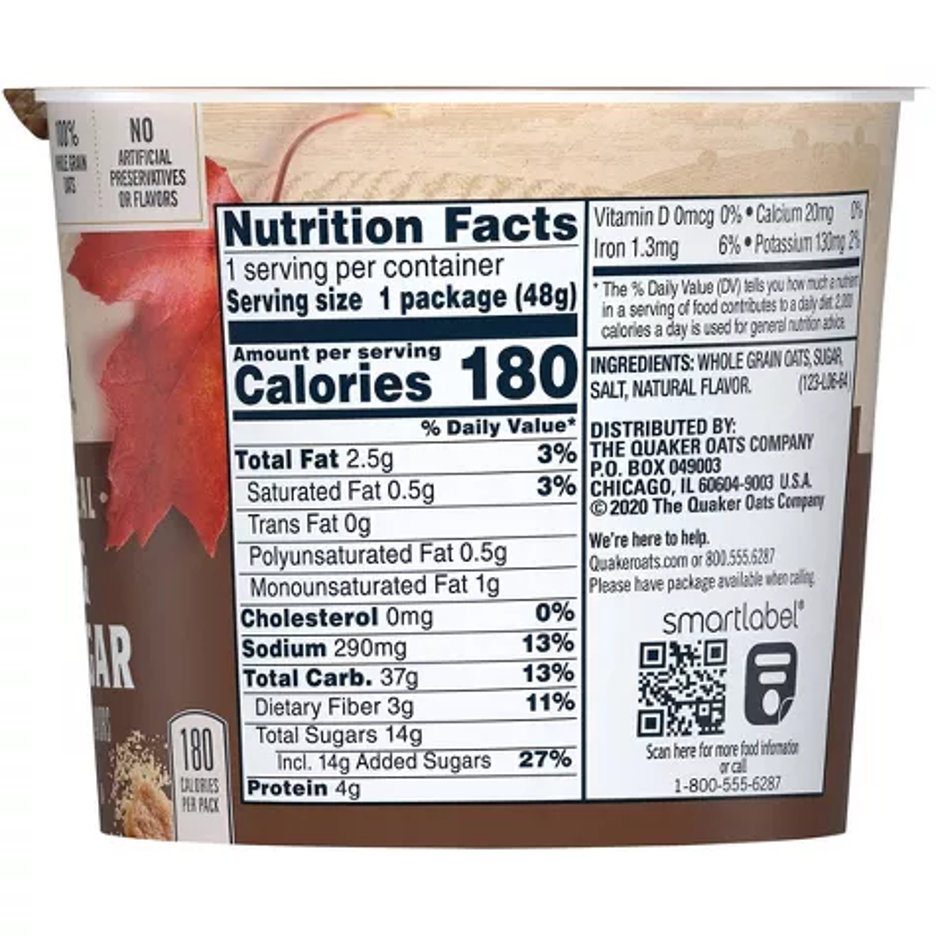
\includegraphics[width=\linewidth]{oatmeal.png}
        \caption{Maple Brown Sugar Oatmeal}
        \label{fig:1}
    \end{subfigure}%
    \begin{subfigure}{0.2\textwidth}
        \centering
        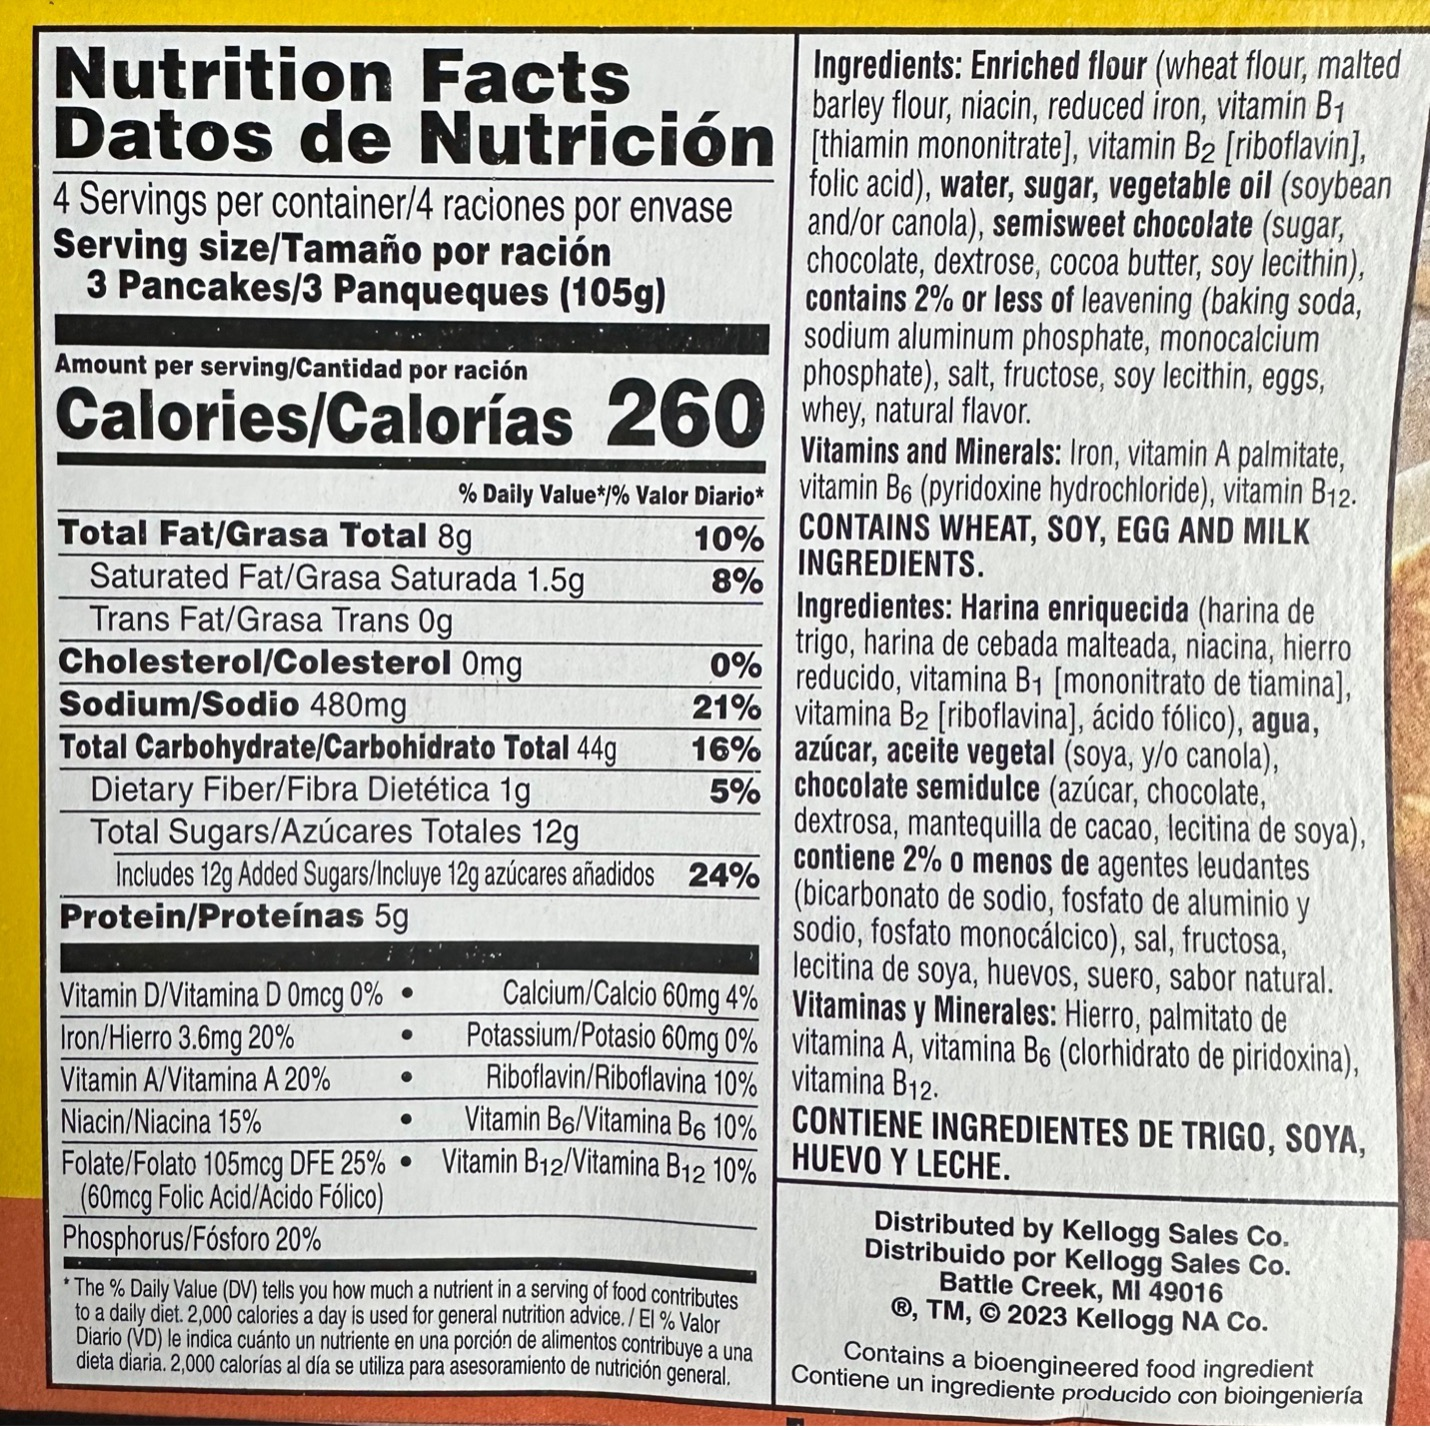
\includegraphics[width=\linewidth]{pancake.jpg}
        \caption{Eggo Chocolate Chip Pancake}
        \label{fig:2}
    \end{subfigure}%
    \begin{subfigure}{0.2\textwidth}
        \centering
        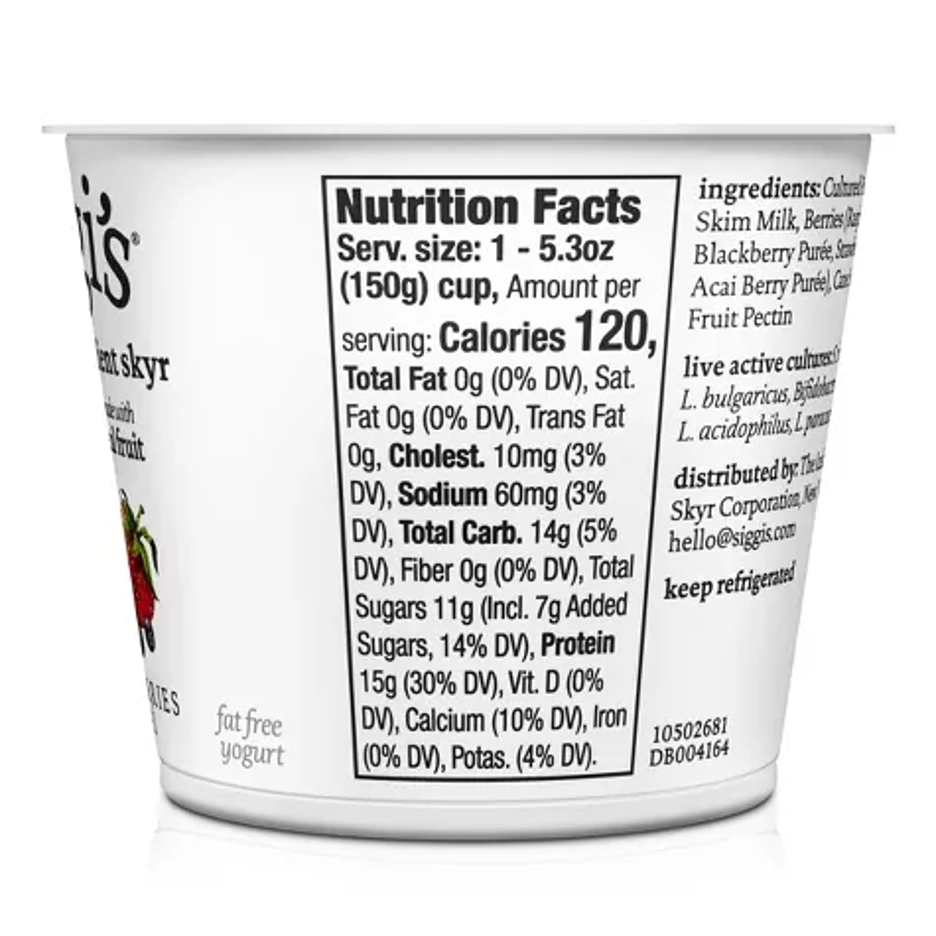
\includegraphics[width=\linewidth]{yogurt.png}
        \caption{Siggi's Yogurt}
        \label{fig:3}
    \end{subfigure}%
    \begin{subfigure}{0.2\textwidth}
        \centering
        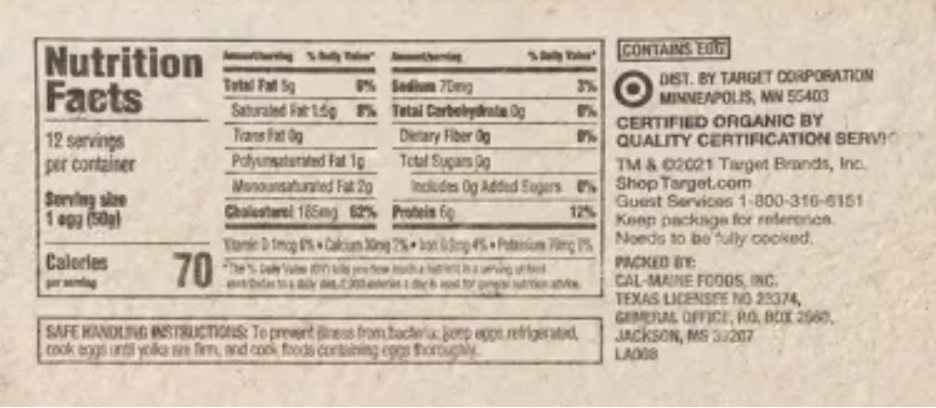
\includegraphics[width=\linewidth]{egg.png}
        \caption{Large Eggs}
        \label{fig:4}
    \end{subfigure}%
    \begin{subfigure}{0.2\textwidth}
        \centering
        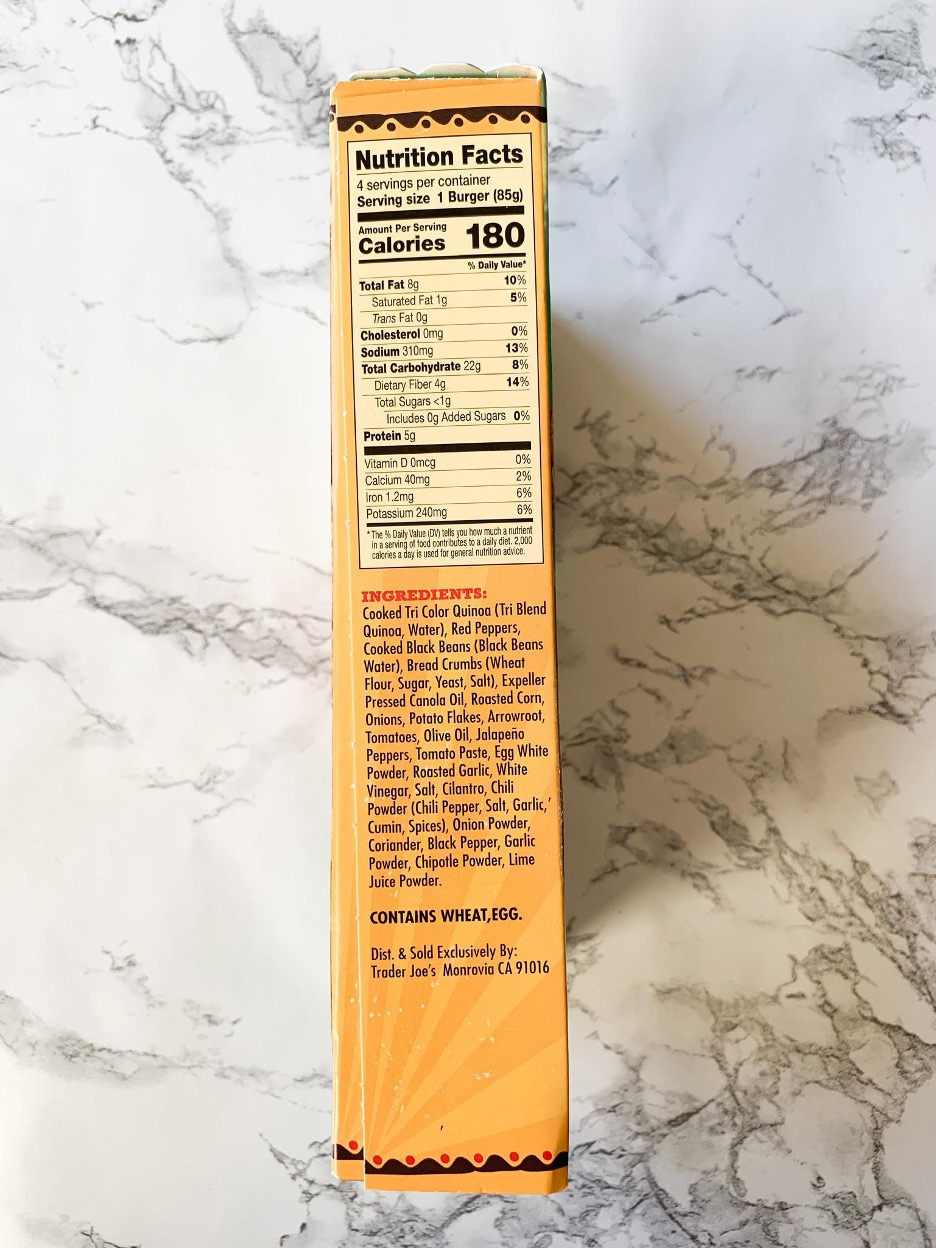
\includegraphics[width=\linewidth]{burger.jpg}
        \caption{Quinoa Cowboy Veggie Burgers}
        \label{fig:5}
    \end{subfigure}
    \caption{Nutrition Facts Labels}
    \label{fig:nutrition_facts}
\end{figure}

\newpage
\subsection{Code Snippets}

\label{Code Snippet - Solution1}
\textbf{Solution 1}
\begin{lstlisting}[language=Python]
from pulp import LpStatus
from pulp import value
from pulp import LpMinimize, LpProblem, LpVariable, lpSum

# Solving the linear programming problem
problem = LpProblem("Personal_Diet_Minimization1", LpMinimize)

# Decision variables representing servings of each food item
oatmeal = LpVariable('Oatmeal', lowBound=0)
pancakes = LpVariable('Pancakes', lowBound=0)
yogurt = LpVariable('Yogurt', lowBound=0)
eggs = LpVariable('Eggs', lowBound=0)
burgers = LpVariable('Burgers', lowBound=0)

# Objective function: minimize total cost
problem += lpSum([0.99 * oatmeal, 0.87 * pancakes, 
                  1.49 * yogurt, 0.42 * eggs, 1.00 * burgers])

# Constraints based on nutritional requirements (weekly)

# Sodium constraint (maximum 35,000 mg per week)
problem += lpSum([290 * oatmeal, 480 * pancakes, 
                  60 * yogurt, 70 * eggs, 310 * burgers]) <= 35000

# Energy constraint (minimum 14,000 kcal per week)
problem += lpSum([180 * oatmeal, 260 * pancakes, 
                  120 * yogurt, 70 * eggs, 180 * burgers]) >= 14000

# Protein constraint (minimum 350 grams per week)
problem += lpSum([4 * oatmeal, 5 * pancakes, 
                  15 * yogurt, 6 * eggs, 5 * burgers]) >= 350

# Vitamin D constraint (minimum 140 mcg per week)
problem += lpSum([0 * oatmeal, 0 * pancakes, 
                  0 * yogurt, 40 * eggs, 0 * burgers]) >= 140

# Calcium constraint (minimum 9,100 mg per week)
problem += lpSum([20 * oatmeal, 60 * pancakes, 
                  130 * yogurt, 30 * eggs, 40 * burgers]) >= 9100

# Iron constraint (minimum 126 mg per week)
problem += lpSum([1.3 * oatmeal, 3.6 * pancakes, 
                  0 * yogurt, 0.9 * eggs, 1.2 * burgers]) >= 126

# Potassium constraint (minimum 32,900 mg per week)
problem += lpSum([130 * oatmeal, 60 * pancakes, 
                  150 * yogurt, 70 * eggs, 240 * burgers]) >= 32900

problem.solve()

optimized_servings = {
    "Oatmeal": oatmeal.varValue,
    "Pancakes": pancakes.varValue,
    "Yogurt": yogurt.varValue,
    "Eggs": eggs.varValue,
    "Burgers": burgers.varValue
}

print(optimized_servings)

print("Status:", LpStatus[problem.status])
for v in problem.variables():
    print(v.name, "=", v.varValue)
print("Total Cost = $", value(problem.objective))
\end{lstlisting}

\textbf{Solution 1 Output}
\label{Solution1 Output}
\begin{lstlisting}[basicstyle=\small]
Welcome to the CBC MILP Solver 
Version: 2.10.3 
Build Date: Dec 15 2019 

command line - /Users/amerchant/anaconda3/lib/python3.11/site-packages/pulp/solverdir/cbc/osx/
64/cbc /var/folders/vk/41zv6b1x0s5g_x9plyd9lt6h0000gn/T/5a68bfb1845f4d4cab353a954f529fd6-
pulp.mps timeMode elapsed branch printingOptions all solution /var/folders/vk/41zv6b1x0s5g_x9plyd9lt
6h0000gn/T/5a68bfb1845f4d4cab353a954f
529fd6-pulp.sol (default strategy 1)
At line 2 NAME          MODEL
At line 3 ROWS
At line 12 COLUMNS
At line 48 RHS
At line 56 BOUNDS
At line 57 ENDATA
Problem MODEL has 7 rows, 5 columns and 30 elements
Coin0008I MODEL read with 0 errors
Option for timeMode changed from cpu to elapsed
Presolve 6 (-1) rows, 5 (0) columns and 29 (-1) elements
0  Obj 1.47 Primal inf 314.21698 (5)
3  Obj 184.2
Optimal - objective value 184.2
After Postsolve, objective 184.2, infeasibilities - dual 0 (0), primal 0 (0)
Optimal objective 184.2 - 3 iterations time 0.002, Presolve 0.00
Option for printingOptions changed from normal to all
Total time (CPU seconds):       0.00   (Wallclock seconds):       0.01

{'Oatmeal': 0.0, 'Pancakes': 0.0, 'Yogurt': 0.0, 'Eggs': 367.14286, 'Burgers': 30.0}
Status: Optimal
Burgers = 30.0
Eggs = 367.14286
Oatmeal = 0.0
Pancakes = 0.0
Yogurt = 0.0
Total Cost = $ 184.20000119999997
\end{lstlisting}

\textbf{Solution 2 with Constraint}
\label{Code Snippet - Solution2}
\begin{lstlisting}[language=Python]
from pulp import LpStatus
from pulp import value
from pulp import LpMinimize, LpProblem, LpVariable, lpSum

# Solving the linear programming problem with a constraints 
problem = LpProblem("Personal_Diet_Minimization2", LpMinimize)

# Decision variables representing servings of each food item
oatmeal = LpVariable('Oatmeal', lowBound=0)
pancakes = LpVariable('Pancakes', lowBound=0)
yogurt = LpVariable('Yogurt', lowBound=0)
eggs = LpVariable('Eggs', lowBound=0)
burgers = LpVariable('Burgers', lowBound=0)

# Objective function: minimize total cost
problem += lpSum([0.99 * oatmeal, 0.87 * pancakes, 
                  1.49 * yogurt, 0.42 * eggs, 1.00 * burgers])

# Sodium constraint (maximum 35,000 mg per week)
problem += lpSum([290 * oatmeal, 480 * pancakes, 
                  60 * yogurt, 70 * eggs, 310 * burgers]) <= 35000

# Energy constraint (minimum 14,000 kcal per week)
problem += lpSum([180 * oatmeal, 260 * pancakes, 
                  120 * yogurt, 70 * eggs, 180 * burgers]) >= 14000

# Protein constraint (minimum 350 grams per week)
problem += lpSum([4 * oatmeal, 5 * pancakes, 
                  15 * yogurt, 6 * eggs, 5 * burgers]) >= 350

# Vitamin D constraint (minimum 140 mcg per week)
problem += lpSum([0 * oatmeal, 0 * pancakes, 
                  0 * yogurt, 40 * eggs, 0 * burgers]) >= 140

# Calcium constraint (minimum 9,100 mg per week)
problem += lpSum([20 * oatmeal, 60 * pancakes, 
                  130 * yogurt, 30 * eggs, 40 * burgers]) >= 9100

# Iron constraint (minimum 126 mg per week)
problem += lpSum([1.3 * oatmeal, 3.6 * pancakes, 
                  0 * yogurt, 0.9 * eggs, 1.2 * burgers]) >= 126

# Potassium constraint (minimum 32,900 mg per week)
problem += lpSum([130 * oatmeal, 60 * pancakes, 
                  150 * yogurt, 70 * eggs, 240 * burgers]) >= 32900

# Add a constraint that requires at least one serving of each food 
problem += oatmeal >= 1
problem += pancakes >= 1
problem += yogurt >= 1
problem += eggs >= 1
problem += burgers >= 1

problem.solve()

optimized_servings = {
    "Oatmeal": oatmeal.varValue,
    "Pancakes": pancakes.varValue,
    "Yogurt": yogurt.varValue,
    "Eggs": eggs.varValue,
    "Burgers": burgers.varValue
}

print(optimized_servings)
print("Status:", LpStatus[problem.status])
for v in problem.variables():
    print(v.name, "=", v.varValue)
print("Total Cost = $", value(problem.objective))
\end{lstlisting}

\textbf{Solution 2 with Constraint Output}
\label{Solution2 Output}
\begin{lstlisting}[basicstyle=\small]
Welcome to the CBC MILP Solver 
Version: 2.10.3 
Build Date: Dec 15 2019 

command line - /Users/amerchant/anaconda3/lib/python3.11/site-packages/pulp/solverdir/cbc/osx/
64/cbc /var/folders/vk/41zv6b1x0s5g_x9plyd9lt6h0000gn/T/5a68bfb1845f4d4cab353a954f529fd6-
pulp.mps timeMode elapsed branch printingOptions all solution /var/folders/vk/41zv6b1x0s5g_x9plyd9lt
6h0000gn/T/5a68bfb1845f4d4cab353a954f
529fd6-pulp.sol (default strategy 1)
At line 2 NAME          MODEL
At line 3 ROWS
At line 17 COLUMNS
At line 58 RHS
At line 71 BOUNDS
At line 72 ENDATA
Problem MODEL has 12 rows, 5 columns and 35 elements
Coin0008I MODEL read with 0 errors
Option for timeMode changed from cpu to elapsed
Presolve 6 (-6) rows, 5 (0) columns and 29 (-6) elements
0  Obj 5.82 Primal inf 303.40331 (5)
2  Obj 188.59
Optimal - objective value 188.59
After Postsolve, objective 188.59, infeasibilities - dual 0 (0), primal 0 (0)
Optimal objective 188.59 - 2 iterations time 0.002, Presolve 0.00
Option for printingOptions changed from normal to all
Total time (CPU seconds):       0.00   (Wallclock seconds):       0.00

{'Oatmeal': 1.0, 'Pancakes': 1.0, 'Yogurt': 1.0, 'Eggs': 386.28571, 'Burgers': 23.0}
Status: Optimal
Burgers = 23.0
Eggs = 386.28571
Oatmeal = 1.0
Pancakes = 1.0
Yogurt = 1.0
Total Cost = $ 188.5899982
\end{lstlisting}
\end{document}
